



\documentclass[
	% -- opções da classe memoir --
	12pt,				% tamanho da fonte
	openright,			% capítulos começam em pág ímpar (insere página vazia caso preciso)
	oneside,			% para impressão em recto e verso. Oposto a oneside
	a4paper,			% tamanho do papel. 
	% -- opções da classe abntex2 --
	%chapter=TITLE,		% títulos de capítulos convertidos em letras maiúsculas
	%section=TITLE,		% títulos de seções convertidos em letras maiúsculas
	%subsection=TITLE,	% títulos de subseções convertidos em letras maiúsculas
	%subsubsection=TITLE,% títulos de subsubseções convertidos em letras maiúsculas
	% -- opções do pacote babel --
	english,			% idioma adicional para hifenização
	french,				% idioma adicional para hifenização
	spanish,			% idioma adicional para hifenização
	brazil				% o último idioma é o principal do documento
	]{abntex2}




% Pacotes básicos 
\usepackage{lmodern}			% Usa a fonte Latin Modern			
\usepackage[T1]{fontenc}		% Selecao de codigos de fonte.
\usepackage[utf8]{inputenc}		% Codificacao do documento (conversão automática dos acentos)
\usepackage{indentfirst}		% Indenta o primeiro parágrafo de cada seção.
\usepackage{color}				% Controle das cores
\usepackage{graphicx}			% Inclusão de gráficos
\usepackage{microtype} 			% para melhorias de justificação
\usepackage{amsmath}			% lib para equacoes
\usepackage{svg}
%\usepackage{float}
\usepackage[T1]{fontenc}
\usepackage{listings}
\usepackage{tikz}
\usepackage{caption}
\usepackage{url}

\usepackage{titlesec}
\newcommand{\sectionbreak}{\clearpage}
\usepackage{hyperref}

\usetikzlibrary{shapes.geometric, arrows}

\tikzstyle{startstop} = [rectangle, rounded corners, 
minimum width=3cm, 
minimum height=1cm,
text centered, 
draw=black, 
fill=red!30]

\tikzstyle{io} = [trapezium, 
trapezium stretches=true, % A later addition
trapezium left angle=70, 
trapezium right angle=110, 
minimum width=3cm, 
minimum height=1cm, text centered, 
draw=black, fill=blue!30]


\tikzstyle{process} = [rectangle, 
minimum width=3cm, 
minimum height=1cm, 
text centered, 
text width=3cm, 
draw=black, 
fill=orange!30]

\tikzstyle{decision} = [diamond, 
minimum width=3cm, 
minimum height=1cm, 
text centered, 
draw=black, 
fill=green!30]
\tikzstyle{arrow} = [thick,->,>=stealth]



\definecolor{dkgreen}{rgb}{0,0.6,0}
\definecolor{gray}{rgb}{0.5,0.5,0.5}
\definecolor{mauve}{rgb}{0.58,0,0.82}

\lstset{frame=tb,
  language=Python,
  aboveskip=3mm,
  belowskip=3mm,
  showstringspaces=false,
  columns=flexible,
  basicstyle={\small\ttfamily},
  numbers=none,
  numberstyle=\tiny\color{gray},
  keywordstyle=\color{blue},
  commentstyle=\color{dkgreen},
  stringstyle=\color{mauve},
  breaklines=false,
  breakatwhitespace=false,
  upquote=true,
  tabsize=3
}

% Pacotes adicionais, usados apenas no âmbito do Modelo Canônico do abnteX2

\usepackage{lipsum}				% para geração de dummy text



% Pacotes de citações
\usepackage[num, backend=biblatex]{abntex2cite}	% Citações padrão ABNT
\usepackage[brazilian,hyperpageref]{backref}	 % Paginas com as citações na bibl

 
% CONFIGURAÇÕES DE PACOTES

% Configurações do pacote backref
% Usado sem a opção hyperpageref de backref
\renewcommand{\backrefpagesname}{Citado na(s) página(s):~}
% Texto padrão antes do número das páginas
\renewcommand{\backref}{}
% Define os textos da citação
\renewcommand*{\backrefalt}[4]{
	\ifcase #1 %
		Nenhuma citação no texto.%
	\or
		Citado na página #2.%
	\else
		Citado #1 vezes nas páginas #2.%
	\fi}%
% ---



% ---
% Informações de dados para CAPA e FOLHA DE ROSTO
% ---
\titulo{Robô omnidirecional de 3 rodas}
\autor{Daniel Ermelino Carvalho \\ Lucas Pereira Lima}
\local{Brasil}
\data{2024}
\orientador{Marcelo Bender Perotoni}
\instituicao{%
  Universidade Federal do ABC
  \par
  CECS
  \par
   Engenharia de Instrumentação, Automação e Robótica}
\tipotrabalho{Trabalho de graduação}
% O preambulo deve conter o tipo do trabalho, o objetivo, 
% o nome da instituição e a área de concentração 
\preambulo{Trabalho apresentado ao curso de engenharia de instrumentação,
automação e robótica da Universidade Federal do ABC como requisito parcial para
obtenção do título de bacharel em Engenharia de Instrumentação, Automação e 
Robótica.}



% Configurações de aparência do PDF final

% alterando o aspecto da cor azul
\definecolor{blue}{RGB}{5,5,180}

% informações do PDF
\makeatletter
\hypersetup{
     	%pagebackref=true,
		pdftitle={\@title}, 
		pdfauthor={\@author},
    	pdfsubject={\imprimirpreambulo},
	    pdfcreator={LaTeX with abnTeX2},
		pdfkeywords={abnt}{latex}{abntex}{abntex2}{trabalho acadêmico}, 
		colorlinks=true,       		% false: boxed links; true: colored links
    	linkcolor=blue,          	% color of internal links
    	citecolor=blue,        		% color of links to bibliography
    	filecolor=magenta,      		% color of file links
		urlcolor=blue,
		bookmarksdepth=4
}
\makeatother


% Posiciona figuras e tabelas no topo da página quando adicionadas sozinhas
% em um página em branco. Ver https://github.com/abntex/abntex2/issues/170
\makeatletter
\setlength{\@fptop}{5pt} % Set distance from top of page to first float
\makeatother



% Possibilita criação de Quadros e Lista de quadros.
% Ver https://github.com/abntex/abntex2/issues/176

\newcommand{\quadroname}{Quadro}
\newcommand{\listofquadrosname}{Lista de quadros}

\newfloat[chapter]{quadro}{loq}{\quadroname}
\newlistof{listofquadros}{loq}{\listofquadrosname}
\newlistentry{quadro}{loq}{0}

% configurações para atender às regras da ABNT
\setfloatadjustment{quadro}{\centering}
\counterwithout{quadro}{chapter}
\renewcommand{\cftquadroname}{\quadroname\space} 
\renewcommand*{\cftquadroaftersnum}{\hfill--\hfill}

\setfloatlocations{quadro}{hbtp} % Ver https://github.com/abntex/abntex2/issues/176


% Espaçamentos entre linhas e parágrafos 


% O tamanho do parágrafo é dado por:
\setlength{\parindent}{1.3cm}

% Controle do espaçamento entre um parágrafo e outro:
\setlength{\parskip}{0.2cm}  % tente também \onelineskip


% compila o indice
\makeindex



% Início do documento
\begin{document}

% Seleciona o idioma do documento (conforme pacotes do babel)
%\selectlanguage{english}
\selectlanguage{brazil}

% Retira espaço extra obsoleto entre as frases.
\frenchspacing 


% ELEMENTOS PRÉ-TEXTUAIS
	
% ---
% Capa
% ---
\imprimircapa
% ---

% ---
% Folha de rosto
% (o * indica que haverá a ficha bibliográfica)
% ---
\imprimirfolhaderosto
% ---



% ---
% inserir o sumario
% ---
\pdfbookmark[0]{\contentsname}{toc}
\tableofcontents*
\cleardoublepage
% ---


% ELEMENTOS TEXTUAIS
\textual

	% Introdução (exemplo de capítulo sem numeração, mas presente no Sumário)
	\chapter{Introdução}

	

Apesar dos diversos desenvolvimentos recentes, pesquisas no campo da robótica móvel são um fenômeno ocorrendo há mais de 50 anos - segundo os padrões atuais, 
o primeiro robô móvel foi o Shakey, desenvolvido entre 1966 e 1972 \cite{TAKAHASHI}. 
Sua principal característica distintiva era a habilidade de perceber arrazoar a respeito de seu entorno, 
sendo capaz de desenvolver tarefas que requeressem planejamento, encontrar rotas e reposicionar pequenos objetos \cite{sri_international}.

À medida em que as técnicas para se construir e controlar robôs móveis (com particular interesse nos robôs móveis autônomos), 
e a isso se somando o fato de que os materiais para sua construção tornaram-se cada vez mais acessíveis (em termos de disponibilidade 
e também de redução de custos), já a partir da década de 80 começaram a surgir robôs autônomos em diversos laboratórios e centros de pesquisa;
 mais recentemente, empresas começaram a comercializar robôs para usuários domésticos, em aplicações como cortadores de grama, aspiradores e pó, 
 e mesmo robôs voltados para entretenimento \cite{TAKAHASHI}.

Robôs são classificáveis diversas maneiras, tais como forma de movimentação, os tipos de tarefas executadas e o seu grau de autonomia, 
bem como agrupando-os entre aquáticos, aéreos e terrestres. A escolha de um dado sistema de locomoção depende de diversas características do robô e 
da tarefa a ser executada, como manobrabilidade, controlabilidade, estabilidade, eficiência e tração \cite{TAKAHASHI}.

Ao se classificar robôs móveis, também é possível se empregar como critério características cinemáticas - particularmente, 
a capacidade do robô se movimentar em qualquer direção. A robôs com restrições em determinados tipos de movimento dá-se o nome de não-holonômicos, 
em oposição a robôs holonômicos, capazes de movimentação em qualquer direção (estritamente, robôs com quantidades de velocidades igual a seu grau de liberdade \cite{TAKAHASHI}).

Em se tratando de robôs terrestres, suas restrições não-holonômicas são consequência direta das rodas empregadas em sua construções. 
Rodas convencionais permitem uma quantidade de movimentos limitada, e, para contornar isso, é possível construir rodas omnidirecionais aos se acrescentar rotores à estrutura de uma roda convencional \cite{TAKAHASHI}.


	% Capitulo com exemplos de comandos inseridos de arquivo externo 
	\include{abntex2-modelo-include-comandos}
	
	\chapter{Objetivos}

\subsection*{Gerais}
Este trabalho tem como objetivos gerais avaliar a viabilidade da utilização de 
um robô omnidirecional de três rodas controlado por microcontrolador para 
atuação independente em ambiente interno.

\subsection*{Específicos}
Deseja-se realizar a construção de um robô a partir de diversos componentes 
(motor, microcontrolador, rodas, driver, chassi, entre outros), e também 
implementar rotina de controle que permita ao robô receber como entrada mapa
do ambiente em que se encontra, de modo que seja capaz de nele se mover de 
acordo com as rotinas desejadas.

	
\chapter{Revisão Bibliográfica}


\section{Veículo omnidirecional de 3 rodas}
Um veículo omnidirecional de 3 rodas no contexto deste trabalho é um robô
holonômico capaz de se mover em translação e rotação simultaneamente e
independentemente \cite{mobile_manipulator_robot}. Sua geometria básica se 
baseia em rodas equidistantes em uma circunferência, com 120° de separação entre
 si, tangenciando o perímetro do chassi do veículo, como demonstrado na figura
 1.

\begin{figure}[ht]
	\centering
	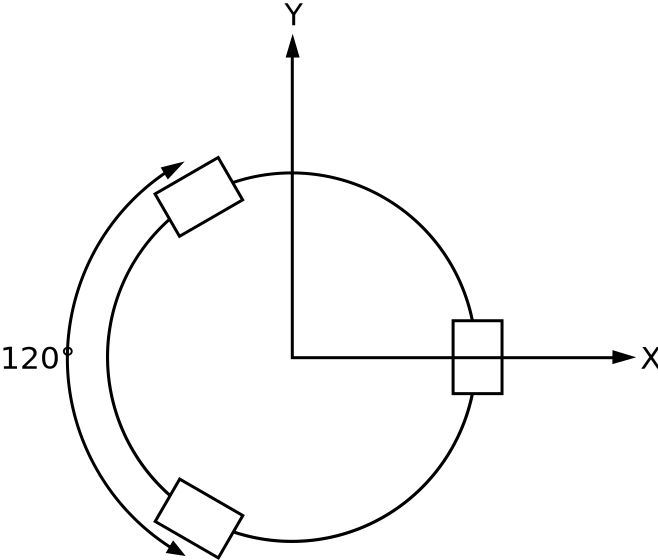
\includegraphics{figures/model}
	\caption{Diagrama do modelo matemático do robô}
\end{figure}

Robôs omnidirecionais tais como esse são particularmente úteis porque permitem
 maior manobrabilidade e eficiência, a um custo de maior complexidade na sua
 construção e controle. \cite{dynamical_models_for_omni_directional_robots}

\subsection{Modelagem Cinemática - Dedução da matriz por cinemática direta}

$\overrightarrow{V}$ é o vetor de velocidade linear do robô, $V_{w1}$, $V_{w2}$,
$V_{w3}$ são as velocidades lineares das rodas 1,2,3. 
$\omega $ é a velocidade angular do robô a partir do seu centro geométrico.
$L$ é a distância entre o centro de geométrico da roda e o centro de geométrico
do robô.


\begin{figure}[ht]
	\centering
	\includegraphics[width=0.8\textwidth]{figures/digram_model_dedution}
	\caption{Diagrama do modelo matemático do robô, com valores dos ângulos das
	rodas}
\end{figure}

\begin{equation}
    \begin{split}
        \overrightarrow{V}_{l} = 
        \overrightarrow{V}_{w1}
        + \overrightarrow{V}_{w2}
        + \overrightarrow{V}_{w3}
    \end{split}
\end{equation}

\begin{equation}
    \begin{split}
        \overrightarrow{\omega} = 
        \frac{\vert\overrightarrow{V}_{w1}\vert}{L}
        + \frac{\vert\overrightarrow{V}_{w2}\vert}{L}
        + \frac{\vert\overrightarrow{V}_{w3}\vert}{L}
    \end{split}
\end{equation}


\begin{gather*}
        V_{l} \angle \theta =  
        V_{w1} \angle \left(-\frac{\pi}{2}\right) 
        + V_{w2} \angle \left(\frac{2\pi}{3}-\frac{\pi}{2}\right) 
        + V_{w3} \angle \left(\frac{4\pi}{3}-\frac{\pi}{2}\right) 
\end{gather*}

\begin{align*}
    V_{l} \cos{ \theta } + jV_{l} \sin{\theta} =  
    V_{w1} \cos{ \left(-\frac{\pi}{2}\right)} + jV_{w1} \sin{ \left(-\frac{\pi}{2}\right) } \\
    + V_{w2}  \cos{ \left(\frac{\pi}{6}\right) } + jV_{w2}  \sin{ \left(\frac{\pi}{6}\right) }  \\
    + V_{w3} \cos{ \left(\frac{5\pi}{6}\right) } + jV_{w2}  \sin{ \left(\frac{5\pi}{6}\right) } 
\end{align*}

\begin{equation*}
    \begin{split}
        \omega = 
        \frac{V_{w1}}{L}
        + \frac{V_{w2}}{L}
        + \frac{V_{w3}}{L}
    \end{split}
\end{equation*}


\begin{gather}
	\begin{bmatrix} V\cdot \cos{\theta} \\  V\cdot \sin{\theta} \\  \omega \end{bmatrix}
	=
	\begin{bmatrix}
		\cos{\left(-\frac{\pi}{2}\right)} & \cos{\left(\frac{\pi}{6}\right)} & \cos{\left(\frac{5\pi}{6}\right)} \\
		\sin{\left(-\frac{\pi}{2}\right)} & \sin{\left(\frac{\pi}{6}\right)} & \sin{\left(\frac{5\pi}{6}\right)} \\
		\frac{1}{L} & \frac{1}{L} & \frac{1}{L}
	\end{bmatrix}
	\cdot
	\begin{bmatrix} V_{w1} \\  V_{w2} \\  V_{w3} \end{bmatrix}
\end{gather}




Matriz da cinemática direta:

\begin{gather}
	\begin{bmatrix}
		\cos{\left(-\frac{\pi}{2}\right)} & \cos{\left(\frac{\pi}{6}\right)} & \cos{\left(\frac{5\pi}{6}\right)} \\
		\sin{\left(-\frac{\pi}{2}\right)} & \sin{\left(\frac{\pi}{6}\right)} & \sin{\left(\frac{5\pi}{6}\right)} \\
		\frac{1}{L} & \frac{1}{L} & \frac{1}{L}
	\end{bmatrix}
	=
	\begin{bmatrix}
		0 & \sqrt{3}/2 & -\sqrt{3}/2 \\
		-1 & 1/2 & 1/2  \\
		1/L & 1/L & 1/L
	\end{bmatrix}
\end{gather}



Matriz inversa:


\begin{gather}
	\begin{bmatrix} V_{w1} \\  V_{w2} \\  V_{w3} \end{bmatrix}
	=
	\begin{bmatrix}
		0 & -2/3 & L/3 \\
		1/\sqrt{3} & 1/3 & L/3\\
		-1/\sqrt{3} & 1/3 & L/3
	\end{bmatrix}
	\cdot
	\begin{bmatrix} V\cdot \cos{\theta} \\  V\cdot \sin{\theta} \\  \omega \end{bmatrix}
\end{gather}


A matriz 3.5 é a matriz de cinemática do robô.
As entradas são o vetor velocidade linear e a velocidade angular do robô, e as
saídas são as velocidades lineares de cada uma das rodas.

Desconsiderando a velocidade angular, é possível observar os vetores velocidades
 das rodas e o vetor velocidade linear do robô na figura \ref{simulacao}, que
 foi gerada por meio de simulação em Python.

\begin{figure}[ht]
	\centering
	\includegraphics[width=0.7\textwidth]{figures/simulacao}
	\caption{Simulação dos vetores}
	\label{simulacao}
\end{figure}

\section{Roda Omnidirecional}
A roda omnidirecional aparece em vários modelos na literatura, tais como no design de J. Graboweicki em 1919 \cite{patent_US1305535A} e o de Josef Blumrich em 1972 \cite{patent_US3789947A}. A roda consiste de rolos perpendiculares à  sua direção de giro, cuja presença tem como efeito conferir à roda a capacidade de se locomover em qualquer direção no seu plano. Essa capacidade é o que confere aos robôs aqui discutidos suas características holonômicas, uma vez que as restrições de movimento a que eles estão sujeitos está normalmente atrelada à construção das rodas \cite{TAKAHASHI}.

\begin{figure}[h]
	\centering
	\includegraphics{figures/omniwheel}
	\caption{Modelo de uma Omniwheel \cite{draw_omniwheel}}
\end{figure}

A relação entre velocidade linear e angular da roda é dada por:

\[V_{w1} = \omega_{w1}\cdot r \] 

em que $V_{w}$ é velocidade linear da roda, $r$ o raio da roda, $\omega_{w} $ e é a velocidade angular da roda.

Uma variação da roda omnidirecional é a roda mecanum, criada por Bengt Ilon \cite{patent_US3876255A} - a diferença entre elas é fundamentalmente a construção dos rolos ligados à estrutura central (que, no caso da roda mecanum, são posicionados a 45°).



\section{Motor DC com encoder e driver para motor}

Um motor DC é fundamentalmente uma máquina elétrica de corrente contínua, que
converte energia elétrica de corrente contínua em energia mecânica. Máquinas
elétricas de corrente contínua são mais fácies de controlar e oferecem uma
grande faixa de velocidades \cite{Maquinas_eletricas}. Devido a essas
características, tornam-se ótimas candidatas para uso em eletrônica e robótica,
pois podem ser usadas com baterias. Para controlar a velocidade de um motor,
é necessário o uso de um encoder, que converte o sinal de posição em um valor
mensurável de velocidade angular.


Para os fins deste trabalho, optou-se pelo uso de um motor DC de 6V 210rpm, 
com taxa de redução de 1:34. O encoder escolhido é um encoder magnético, já
vem acoplado ao motor empregado, com 11 PPR (\textit{Pulses Per Revolution}).

\subsection{Encoder magnético}

Por se utilizar um encoder PRR, são produzidas duas ondas quadradas como saídas,
A e B \cite{encoder_ppr}. As duas possuem 90° de fase entre si, e, caso a onda A
esteja adiantada em relação a B (\ref{encoder_ppr_ab}), o sentido de rotação é
positivo (anti-horário).

\begin{figure}[h]
	\centering
	\includegraphics[width=0.6\textwidth]{figures/encoder_holzer}
	\caption{Encoder holzer \cite{encoder_holzer}}
\end{figure}

\begin{figure}[h]
	\centering
	\includegraphics[width=0.7\textwidth]{figures/encoder_pulso_ab}
	\caption{Ondas quadradas resultantes dos pulsos de saída do encoder \cite{encoder_ppr}}
	\label{encoder_ppr_ab}
\end{figure}




\section{Microcontrolador STM32}
O STM32F103C8, também conhecido como Blue Pill, é um microcontrolador fabricado pela STMicroelectronics, de 32-bits, tem como processador o ARM Cortex-M3, de 64Kbs de memória flash.
O processador Cortex-M3, projetado pela ARM (Advanced RISC Machine Ltd.) é  baseado em arquitetura Harvard, de 32-bits.
A família de microcontroladores STM32 fornece uma base par uma uma granda variedades de sistemas embarcados,  e com custo porém essa flexibilidade e custo menor em comparação ao Arduino com o ATmega, que possui microcontroladores de 8 a 16bits.
Porém essa flexibilidade e baixo custo poissui requer um nível de experiência maior em programação C comparado ao Arduino, que foi pensado para ser mais amigável com iniciantes \cite{cortex_m3}.
O STM32F103C8 possui 7 timers, 2 ADCs, e 9 interfaces de comuinicação, incluindo I2C (Inter-Integrated Circuit), USART (Universal Synchronous Asynchronous Receiver Transmitter), SPI (Serial Peripheral Interface), CAN e USB 2.0


\begin{figure}[h]
	\centering
	\includegraphics[width=1.0\textwidth]{figures/stm32f1_pinout}
	\caption{Diagrama de pinos do STM32F103C8}
\end{figure}



\section{IDE}
A IDE a ser usada para programar um STM32 é o TrueSTUDIO, distribuído pela
Atollic, que foi adquirida pela STMicroelectronics em 2017. Trata-se de um
software livre para programar em C/C++, criado com base na plataforma Eclipse,
e que possui todas as funções esperadas para o trabalho com o STM32, tais como
edição, compilação e debug. Uma de seus principais vantagens é não haver
limites para tamanho de projeto, o que o torna ideal para trabalhos
profissionais. O TrueSTUDIO deixou de receber atualizações em 2017,
depois da aquisição pela STMicroelectronics.\cite{apostila_microprossados}

\begin{figure}[h]
	\centering
	\includegraphics[width=0.8\textwidth]{figures/atollic}
	\caption{Interface Atollic \cite{apostila_microprossados}}
\end{figure}



\section{CAD - Design auxiliado por computador}
CAD é a sigla para "computer-aided design", design auxiliado por computador, e pode ser definido como o uso de sistemas computadorizados (hardware + software)
para criação, modificação, análise ou otimização do design \cite{computer_aided_esign}.
O software CAD consiste em um programa capaz de implementar gráficos computadorizados e aplicar funções como análise tensão-deformação de componentes, resposta dinâmica de mecanismos,
cálculos de transferência de calor. As aplicações variam conforme a necessidade da área.

\subsection{AutoCAD}
AutoCAD foi criado em 1982, seu uso mais popular é em desenhos arquitetônicos, mas também tem um forte uso na criação de desenhos técnicos.

\begin{figure}[h]
	\centering
	\includegraphics[width=1\textwidth]{figures/autocad_screen}
	\caption{Interface do AutoCad}
	\label{fig:interface_autocad}
\end{figure}

\subsection{SolidWorks CAD 3D}
Com um foco maior em projetos de engenharia, esse software CAD tem um foco na criação do modelo 3D das peças, considerando precisão de medidas e materiais.
O pacote de softwares adicionais oferece simulações de elementos finitos como análise térmica, vibrações, queda, dinâmica, pressão entre outros.

\begin{figure}[h]
	\centering
	\includegraphics[width=1\textwidth]{figures/soliworks}
	\caption{Interface do SolidWorks}
	\label{fig:interface_soliwoks}
\end{figure}

\section{Impressão 3D de filamento - Manufatura Aditiva}
A manufatura aditiva é o processo de fabricação a partir de adição de camadas de materiais com base em dados de
CAD-3D \cite{manufatura_aditiva}. Manufatura aditiva é o nome que se dá para impressão 3D, se constituindo como
terceiro pilar na tecnologia de manufatura, que inclui também a "manufatura subtrativa" (mais conhecido como processos
de usinagem) e a "manufatura formativa" (como fundição, injeção e conformação).

Como ilustrado na figura \ref{fig:manufatura_aditiva}, asas etapas típicas da manufatura aditiva são:

\begin{enumerate}
	\item Obtenção do modelo CAD 3D;
	\item Fatiamento do modelo e obtenção o contorno das camadas;
	\item Adição de camadas de materiais;
	\item Obtenção do produto final.
\end{enumerate}

O modelo é fatiado por meio de um software, e o resultado é geralmente um conjunto de contornos de mesma espessura.
Esse conjunto de contornos é convertido em comandos a serem executados por uma máquina, em ações de processamento das
camadas. No caso de uma impressora 3D de filamento, o software que obtém as informações de camadas converte essas
informações em código G, linguagem padronizada para máquinas CNC.

\begin{figure}[h]
	\centering
	\includegraphics[width=1\textwidth]{figures/manufatura_aditiva}
	\caption{Processo de manufatura aditiva \cite{manufatura_aditiva}}
	\label{fig:manufatura_aditiva}
\end{figure}


	
\chapter{Metodologia}

Para a execução deste projeto, optou-se pelo uso de componentes amplamente disponíveis no mercado a relativamente baixo
custo, bem como software disponível gratuitamente no site do fabricante. Essas escolhas visam facilitar a
reproducibilidade do projeto, bem como tornar o resultado final do projeto mais eficiente, produzindo o resultado
desejado com o menor custo. 

Um outro fator relevante que impactou a escolha dos componentes a serem utilizados no projeto é a compatibilidade entre
eles - seja ela mecânica, eletrônica ou mesmo de software. Diferentemente de uma solução completa oferecida por
um só fabricante, em que há garantia de operação harmoniosa entre os componentes, este trabalho envolveu a composição de
diferentes partes, pelo que se tornou necessário avaliar a viabilidade de se utilizar todas elas em conjunto.

Ainda assim, dada a necessidade de se utilizar peças com formatos e dimensões específicas para a aplicação em questão,
optou-se também pelo uso de técnicas de impressão 3D. Essa decisão é compatível com o objetivo geral de baixos custos, e
também resolve problemas relacionados à montagem mecânica.


\section{Hardware}
A aquisição dos componentes de hardware empregados neste projeto se deu, em boa parte, por meio de lojas importadoras de
componentes. Optou-se por componentes de baixo custo e, ao mesmo tempo, comumente utilizados em projetos dessa natureza,
a fim de se ter amplo apoio da comunidade na resolução de eventuais problemas encontrados no desenvolvimento da solução.
A tabela \ref{custos} apresenta os custos de cada componente de hardware adquirido para uso exclusivo neste projeto
(excluindo, portanto, equipamentos empregados mas não utilizados apenas nele, como a impressora 3D).


\begin{quadro}[htb]
	\caption{Lista de componentes, materiais e seus custos - valores em reais (R\$) \label{custos}}
	 \begin{tabular}{|c|c|c|c|}
		\hline
		\textbf{Componente ou Material} & \textbf{Valor unitário} & \textbf{Quant} & \textbf{Valor Total} \\ \hline
		Driver Ponte H L298N \cite{l298n_produto} &  22,90 & 3 &  68,70   \\ \hline
		Motor DC 6V 210 RPM \cite{motor_dc_6v_produto} &  90,00 & 3 &  270,00   \\ \hline
		Filamento PLA \cite{filamento_pla_produto} &  99,99 & 1 &  99,99   \\ \hline
		Kit 4 rodas Omnidirecional \cite{omin_wheel_produto} &  131,35 & 1 &  131,35   \\ \hline
		Kit 4 peças eixo roda \cite{omin_wheel_produto} &  42,15 & 1 &  42,15   \\ \hline
		STM32 (microcontrolador) \cite{stm32_produto} &  46,90 & 1 &  46,90   \\ \hline
		Bateria selada 6V \cite{bateria_6v_produto} &  69,90 & 1 &  69,90  \\ \hline
		Powerbank &  119,90 & 1 &  119,90   \\ \hline
		Paquímetro  &  49,90 & 1 &  49,90   \\ \hline
		Ferro de solda &  43,20 & 1 &  43,20   \\ \hline
		Solda &  12,99 & 1 &  12,99   \\ \hline
		Conector mjjst macho &  4,90 & 3 &  14,70   \\ \hline
		Conector mjjst femea &  4,90 & 3 &  14,70   \\ \hline
		Garra jacaré &  1,65 & 2 &  3,30   \\ \hline
		Driver Ponte H DTV8833 \cite{drv8833_produto} &  15,00 & 3 &  45,00   \\ \hline
		Módulo Bluetooth \cite{hc05_produto} &  35,00 & 1 &  35,00   \\ \hline
		Mini Protoboard &  5,00 & 2 &  10,00   \\ \hline
		Protoboard 830 &  16,00 & 1 &  16,00   \\ \hline
		Jumper macho-macho &  8,00 & 1 &  8,00   \\ \hline
		Pasta de solda &  14,99 & 1 &  14,99   \\ \hline
		Sugador de solda &  12,99 & 1 &  12,99   \\ \hline	
		\textbf{CUSTO TOTAL} & & & \textbf{ 1.129,66}   \\ \hline
	\end{tabular}
\end{quadro}

\subsection{Componentes eletrônicos}

\subsubsection{Motor de passo}

Para a execução deste projeto, foi pensado inicialmente o uso de motores DC,  devido a facilidade de uso.
Como os motores DC variam a velocidade com base na tensão disponível, tornando o acionamento simples.
Porém o controle de velocidade é mais complexo, fazendo o uso de encoders.
A leitura dos resultados do encoders possuem muitos ruidos de medição e variam muito com a frequência de amostragem, 
mas remover os ruidos de alta frequência do sinal possa ser resolvido usando um algorítimo de filtro passa baixa discreto.
Porém os motores DC tem a limitação de trabalharem em uma faixa de rpm específica, podendo o motor não alcançar um rpm mínimo desejado.
Um motor de 6v/210 RPM usado tinha baixo torque a baixas velocidades, além de precisar de uma corrente de partida mais alta do que a tensão inicial fornecia.
Trocar por motores de menor velocidade acabaria tendo o problema de não ser possível alçarem um velocidade mais alta quando necessário.
Para usar um motor DC com uma boa variação de velocidade, seria necessário usar um conjunto de engrenagens para obter o rpm desejado sem grandes perdas de torque nos motores
e sem problemas de corrente de partida insuficiente.

Devido essas limitações se optou por motores de passo,  nema 17 bipolar, de uso padrão em impressoras 3D.
A escolha foi motivada pela facilidade de aquisição e maior disponibilidade no mercado, tornando o preço mais baixo do que motores DC,
Em média os valores de um Nema 17 chegam a metade do valor de um motor DC de baixo RPM.
Outro motivo que levou a escolha, foi o fato de serem motores de reposição de uma impressora 3D usada no projeto.

Pelo fato de motor de passo ser controlado em passos por segundo, o controle de velocidade é mais fácil,
e as possíveis variações de rpm ocorrem a nível de ciclos do microcontrolador.

Porém motores de passo exigem um cuidado maior, além de exigem uma alimentação maior, de 12v a 24v, os uso dos drivers para motor de passo exigem um maior cuidado na montagem.

\begin{figure}[htb]
	\centering
	\includegraphics[width=0.7\textwidth]{figures/JK42HS40_1704_13A}
	\caption{Motor de passo Nema 17 \cite{motor_dc_6v_encoder}}
\end{figure}

\begin{quadro}[htb]
\caption{\label{Especificacoes_motordc_6v}Especificações do motor DC 6V}
	 \begin{tabular}{|c|c|c|c|}
		\hline
		\textbf{Especificação} & \textbf{Valor} \\ \hline
		Corrente por fase & 1.7A  \\ \hline
		Torque nomimal  & 4.2 KGF (~46 N) \\ \hline
		Angulo de passo & 1.8° \\ \hline
		Polaridade & bipolar \\ \hline
	\end{tabular}
	\fonte{\cite{chinhai_motor}}
\end{quadro}


Outro desafio do motor de passo é idenfiticar as fases, pois cada fabricante pode ter uma ordem diferente dos pinos de saida do motor.
Para idenfiticar quais pinos compõem cada fase, bastou verificar com o multimetro quais fases estavam em curto.
Restando identicar somente o pontos A e B de cada fase de acordo com o diagrama a seguir.

\begin{figure}[htb]
	\centering
	\includegraphics[width=0.7\textwidth]{figures/motor_wiring}
	\caption{Motor de passo - Fases Bipolar \cite{motor_dc_6v_encoder}}
\end{figure}

Para identificar quais eram os pontos A e B de cada fase, foi necessário um processo de tentantiva e erro,
para relacionar o diagrama de fases com os pinos do motor, e o resultado esta ilustrado na figura \ref{nema_pinout}

\begin{figure}[htb]
	\centering
	\includegraphics[width=0.7\textwidth]{figures/motor_pinout}
	\caption{Motor de passo - Idetificação dos pinos  \cite{motor_dc_6v_encoder}}
	\label{nema_pinout}
\end{figure}



\subsubsection{Driver de Motor}

Diferente de um driver de motor DC, como o L289N e o DRV8833, que rececem um sinal PWM e convertem propocionalmente
para o sinal de tensão a ser aplicado no motor,  os driver de motor de passo são responsáveis por aplicar uma corrente constante, independende da tensão de alimentação.
sendo essa podendo variar de acordo com os limites dos motores e do próprio driver,  por convensão, para um Nema 17, é comnum se trabalhar com uma alimentação
de 12v a 24v.

O driver DRV8825 exige alguns cuidados, alguns informados em documentação e outros não.
Um dos cuidado a ser informado é o ajuste do Vref, nas documentações é dito que é necessário apenas ligar a alimentação dos motores e o ground do microcontrolador
porém em vários testes, alguns drivers pararam de funcionar,  foi então encontrado em fóruns que é recomendado que a carga (o motor) esteja ligado durante esse processo de ajuste do Vref
e que e nenhuma hipotese o driver deve ser alimentado sem que a carga esteja conectada.


\begin{figure}[htb]
	\centering
	\includegraphics[width=0.7\textwidth]{figures/DRV8825}
	\caption{Driver Ponte H DVR8833 \cite{DRV8833_image}}
\end{figure}


\subsubsection{Microcontrolador}

Inicialmente foi escolhido o STM32F103C8, porém a comunicação serial via microusb não pode ser usada ao mesmo tempo que
a alimentação de 3.3v do gravador ST-link. isso pode causar danos no controlador. Por causa dessa limitação foi escolhido o ESP32 DevKit v1.
Embora  quantidade de pinos disponíveis seja menor, não será necessário o uso de pinos de comunicação serial para usar com um módulo bluetooth,
já que o ESP32 já possui bluetooth integrado.

De acordo com o datasheet do ESP32 \cite{esp32_datasheet} e a análises disponíveis online de entusiastas do uso do ESP32 \cite{esp32_reference},
existem alguns pinos recomendados para se usar, alguns que requerem atenção no uso, e outros que recomendam evitar.

\begin{figure}[htb]
	\centering
	\includegraphics[width=1.0\textwidth]{figures/esp32_pinout}
	\caption{Diagrama de pinos do ESP32 Devkit v1 \cite{esp32_reference}}
\end{figure}


\begin{figure}[htb]
	\centering
	\includegraphics[width=0.35\textwidth]{figures/esp32_pinout_ref}
	\caption{Recomendação de uso dos pinos do ESP32 Devkit v1 \cite{esp32_reference}}
\end{figure}


\subsubsection{Alimentação}
Para alimentar o microcontrolador, um powerbank com saída de 5V foi empregado usado, considerando que o STM32F103C8 
funciona a uma corrente abaixo de 100mA. Para alimentar os motores, durante o desenvolvimento, optou-se por uma 
bateria de chumbo-ácido de 6V 4.5Ah.


\subsection{Fabricação e montagem}
O chassi e demais peças foram fabricados por meio de impressão 3D, usando filamento de PLA (ácido poliáctico). As
peças foram projetadas no AutoCAD, e posteriormente modeladas em 3D com o SolidWorks. A geometria do modelo
resultante de cada peça foi convertida em código G para uma impressora 3D por meio do software UltiMaker Cuda. Por
fim, a impressão das peças foi realizada em uma impressora Ender 3 S1 Pro.



% \subsection{Joystick de controle}
% Um joystick de 3 eixos para controlar o robô para testar a cinemática de movimento.
% {\color{red} É necessário aqui especificar o modelo utilizado e descrever características.}

% \subsection{Sensores}
% {\color{red} Esta subseção deve descrever os sensores utilizados e também sua finalidade.}

% \subsection{Dispositivos de comunicação}
% {\color{red} Esta subseção deve descrever os dispositivos de comunicação utilizados (Wi-fi, Bluetooth, etc) e também sua
% finalidade.}

% \subsection{Calibração de parâmetros}
% {\color{red} Caso haja necessidade de calibração de parâmetros de alguns dos componentes utilizados (sensibilidade de
% sensores, histerese de componentes mecânicos, taxa de comunicação de dispositivos, etc), os procedimentos devem ser
% descritos nesta subseção.}

\section{Software}
Para controlar o robô, inicialmente foi pensando em usar uma aplicação drag\&drop para criar um app andriod que envia dados via bluetooth serial.
Porem realizando um benchmark de outros app disponíveis para interações bluetooth com arduino optamos por usar dois desses app e usar de uma maneira diferente.


\subsection{Programação do microcontrolador}
Nesta aplicação, o microcontrolador contém é responsável por coordenar a operação do robô. Por essa razão, foi
necessário programar tal funcionalidade em sua memória. Neste processo, foi necessário configurar os diferentes pinos de
entrada segundo suas capacidades e o uso desejado no projeto, bem como implementar o processamento dos sinais de entrada
(referentes à velocidade dos motores) e a produção de saída (valores a serem enviados como variável manipulada para os
motores do robô). É também do microcontrolador a tarefa de interpretar os comandos recebidos via Bluetooth pelo módulo 
HC-05 (e transmitidos ao STM32 via comunicação serial) e convertê-los em sinal de controle.

\subsection{Aplicativo Android}

O aplicativo Arduino Bluetooth Controller possui uma opção em que o aplicativo envia uma 'string' representando as cores RGB em 'int8'.
por exemplo,  vermelho seria '255000000' (r=255, g=0, b=0). E a interface é o modelo de cor HSV em 2 dimensões de ponta cabeça,
figura \ref{arduino_bluetooth_controller_hsl_model}.


\begin{figure}[htb]
	\centering
	\includegraphics[width=0.40\textwidth]{figures/andriod_bluetooth_controller_hsl_model}
	\caption{Tela de controle RGB do aplicativo Arduino Bluetooth Controller}
	\label{arduino_bluetooth_controller_hsl_model}
\end{figure}

No modelo HSV,  figura  \ref{rbg_hsl_hsv}, 'H' significa "hue" ou matiz, e é um valor do angulo no modelo HSV, 'S' significa 'saturação' e corresponde a um valor de raio,
por último, 'V' é valor, que corresponde a uma terceira dimensão, que não aparece no modelo bidimensional disponível no aplicativo.
Exitem outros dois modelos parecidos que usam a mesma representação cilíndrica, HSL, e HSB, que possuem uma lógica semelhando ao HSV.


\begin{figure}[htb]
	\centering
	\includegraphics[width=0.6\textwidth]{figures/RBG_HSL_HSV}
	\caption{Modelos RGB, HSL e HSV \cite{rbg_hsl_hsv}}
	\label{rbg_hsl_hsv}
\end{figure}

\begin{figure}[htb]
	\centering
	\includegraphics[width=0.8\textwidth]{figures/HSV}
	\caption{Modelo HSV bidimensional \cite{hsv_model}}
\end{figure}


O aplicativo retorna os valores em RGB, então usando um algorítimo que converte RGB para HSV e invertendo o eixo Y
é possível ter os valores de angulo e módulo de um vetor velocidade.
As imagens \ref{hsv_exemplo_1} e \ref{hsv_exemplo_2} possuem os seguintes valores de RGB, que aplicados no algorítimo de conversão geram os resultados no quadro :

\begin{figure}[htb]
	\centering
	\includegraphics[width=0.9\textwidth]{figures/example_1_arduino_color}
	\caption{Modelo HSV bidimensional exemplos n1}
	\label{hsv_exemplo_1}
\end{figure}

\begin{figure}[htb]
	\centering
	\includegraphics[width=0.9\textwidth]{figures/example_2_arduino_color}
	\caption{Modelo HSV bidimensional exemplos n2}
	\label{hsv_exemplo_2}
\end{figure}

\begin{quadro}[htb]
	\caption{\label{HSV_resultado}Resultado algoritmo}
		 \begin{tabular}{|c|c|c|}
			\hline
			\textbf{RGB} & \textbf{Ângulo} & \textbf{Magniture} \\ \hline
			196, 115, 255 & 275.0 & 54.9\% \\ \hline
			131, 143, 255 & 234.0 & 48.63\% \\ \hline
			123, 255, 245 & 175.0 & 51.76\% \\ \hline
			105, 255, 159 & 142.0 & 58.82\% \\ \hline
			198, 255, 124 & 86.0 & 51.37\% \\ \hline
			255, 251, 115 & 58.0 & 54.9\% \\ \hline
			255, 101, 107 & 358.0 & 60.39\% \\ \hline
			255, 142, 247 & 304.0 & 44.31\% \\ \hline
			001, 000, 255 & 240.0 & 100.0\% \\ \hline
			000, 255, 242 & 177.0 & 100.0\% \\ \hline
			000, 255, 023 & 125.0 & 100.0\% \\ \hline
			130, 255, 000 & 89.0 & 100.0\% \\ \hline
			255, 244, 000 & 57.0 & 100.0\% \\ \hline
			255, 000, 005 & 359.0 & 100.0\% \\ \hline
			254, 000, 255 & 300.0 & 100.0\% \\ \hline
		\end{tabular}
	\end{quadro}

Por meio do uso da plataforma MIT App Inventor, vou possível simplificar significativamente o desenvolvimento de um app
Android para uso neste trabalho. A plataforma fornece elementos visuais para produção da interface do app, bem como 
permite implementação de algumas funcionalidades mais comuns (como acesso à comunicação Bluetooth de um Smartphone) a 
serem associadas com esses elementos visual. A app desenvolvido tem por objetivo enviar comandos simples, relacionados
a direções a serem seguidas pelo robô, como demonstra figura \ref{fig:mit_app_inventor}.

\begin{figure}[htb]
	\centering
	\includegraphics[width=0.5\textwidth]{figures/mit_app_inventor.png}
	\caption{Interface da plataforma MIT App Inventor}
	\label{fig:mit_app_inventor}
\end{figure}
	
	

\chapter{Desenvolvimento}

\section{Resposta do robô a estímulos}
{\color{red} Esta seção busca descrever o desempenho do controle sobre os atuadores do robô - dados comandos diretos ao
robô, quão próxima é a sua resposta ao valor desejado.}

\section{Interação com ambientes internos}
{\color{red} Esta seção busca descrever como o robô se comporta ao receber mapas de ambientes internos no formato 
escolhido: quão capaz é o robô de seguir rotinas, responder aos estímulos dos seus sensores corretamente, etc}

\section{Oportunidades de melhoria para trabalhos futuros}
{\color{red} Esta seção dedica-se a descrever o que não foi possível atingir nesta trabalho, e procura sugerir
abordagens e técnicas alternativas para melhor atingimentos dos objetivos estabelecidos anteriormente, ou mesmo sua
sua superação, atingindo níveis de funcionalidade além dos previstos no escope deste projeto.}

	
\chapter{Próximas etapas}

\section{Controle PID em motor DC}
Após lidar com o problema da não linearidade da respostado do motor ao sinal PWM
o próximo passo em controlar a velocidade é a implementação do controle PID.
O desafio será controlar a posição no tempo, considerando a velocidade resultante do robô.

\section{Integração bluetooth}
Para testar a cinematica do robô, iremos controla-lo via bluetooth. Para isso falta implementar a 
leitura via serial usando protocolo UART.

\section{Teste com motor de passo de alto torque - bj42d15}
Foi considerado trocar o tipo de motor e fazer um compartivo entre os diferentes tipos de 
controle e implementação necessário para cada tipo de motor,
e apontar as diferenças de resultados.
Foi sugerido usar o motor de passo bj42d15, comum em impressoras 3d,
que possui um torque mais alto e bons resultados no uso de equipamentos que exigem precisão de posicionamento.

	\chapter{Controle velocidade}

\section{Medição de velicidade do motor}

Como encoder possuí dois sinais de onda quadadra defasadas em 90º, fase A e fase B, cujos vales e picos são valores lógicos HIGH e LOW, 
e direção de rotação do motor pode ser definida pela diferença entre as fases, se fase A esta adiantada ou atrasada em relação a fase B
É possível calcular a velocidade com base nas subidas da onda quadrada de uma fase, e o valor logico da outra fase no momento da subida.
Por exemplo,  observando a fase B, toda vez em que há uma subida, se o valor da fase A for alto, então incrementar +1 em um contador, se a fase A tiver valor baixo, então incrementar -1 no contador.
Quando o valor da fase A for alto, então o motor esta rodando em um sentido,  quando o valor  for baixo, então o motor esta rodando no sentido contrário.
Medindo o valor do contador por um $\Delta_{T}$, se resulta na quantidade de pulsos por segundo.
Para converter de pulsos por segundo para RPM, basta dividir pela resolução do motor+encoder,  que é de 1:34 do motor, e 11 pulsos por rotação do encoder, o que resulta em 374,
e multiplicar por 60 para ter o resultado em rotações por minuto.


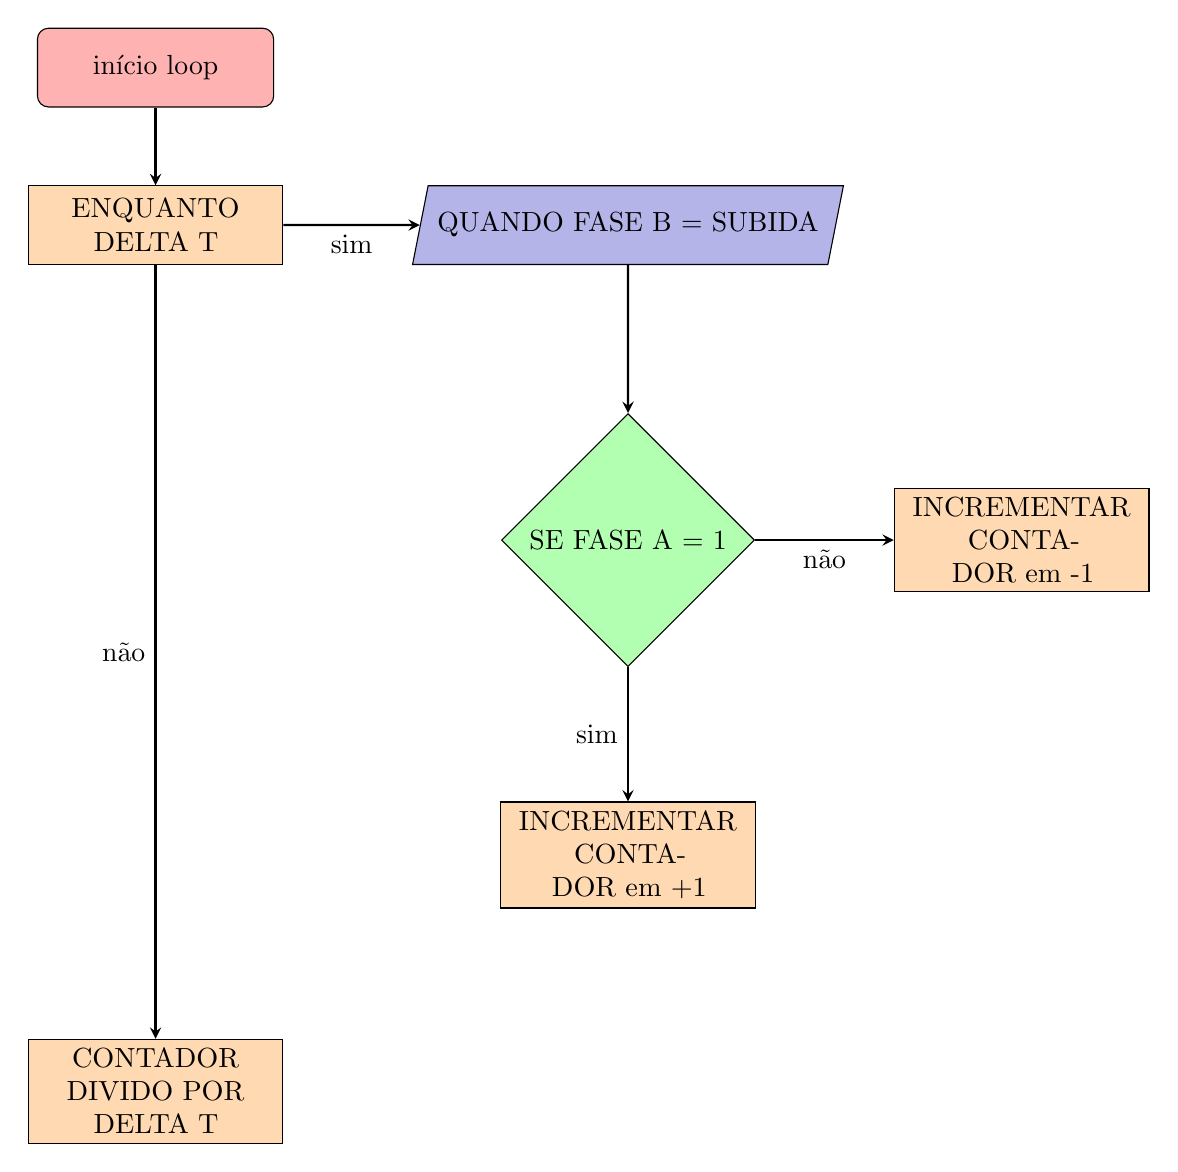
\begin{tikzpicture}[node distance=2cm]

    \node (start) [startstop] {início loop};
    \node (pro1) [process, below of=start] {ENQUANTO DELTA T};
    
    \node (in1) [io, right of=pro1, xshift= 4cm] {QUANDO FASE B = SUBIDA};
    
    \node (dec1) [decision, below of=in1, yshift=-2cm] {SE FASE A = 1};
    \node (pro1a) [process, below of=dec1, yshift= -2cm] {INCREMENTAR CONTADOR em +1};
    \node (pro1b) [process, right of=dec1, xshift= 3cm] {INCREMENTAR CONTADOR em -1};
    
    
    \node (count) [process, below of=pro1, yshift= -9cm] {CONTADOR DIVIDO POR DELTA T};
    
    \draw [arrow] (start) -- (pro1);
    \draw [arrow] (pro1) -- node[anchor=north] {sim} (in1);
    \draw [arrow] (in1) -- (dec1);
    \draw [arrow] (dec1) -- node[anchor=east] {sim} (pro1a);
    \draw [arrow] (dec1) -- node[anchor=north] {não} (pro1b);
    
    \draw [arrow] (pro1) -- node[anchor=east] {não} (count);
    
\end{tikzpicture}
    


Na implementação dessa lógica no STM32, o desafio foi a definição do $\Delta_{T}$,
Se o $\Delta_{T}$ for muito pequeno, o resultados de pulsos por segundo pode tender ao infinito, gerando valores muito altos.
Na figura \ref{fig:medidas_altas} em laranja, esta o resultado do rpm considerando o $\Delta_{T}$ como o tempo entre os ciclos do micrcontrolador.
A outra opção, foi definir um $\Delta_{T}$ fixo, definindo uma frequencia de medição pré definida, e o resultado pode ser visto em azul na figura \ref{fig:medidas_altas}
Essa outra opção de $\Delta_{T}$ resultou em um sinal que tem uma componente em alta frequência com uma amplitude até consideral.
Analisando os dois sinais no dominio da frequêcia na figura \ref{fig:frequencia_medidas_altas}, o espectro em frequência do sinal em laranja possui amplitudes muitos semelhante em todo espectro, mas o espectro do sinal em azul, fica bem claro que em altas frequencias é composto mais por ruidos
e as frequencia médias tem amplitude menor em relação as frequências baixas, o que torna mais fácil aplicar um filtro passa-baixa para reduzir as frenquências médias e altas.


\begin{figure}[h]
	\centering
	\includegraphics{figures/medidas_altas}
	\caption{Problemas com delta T muito pequeno}
	\label{fig:medidas_altas}
\end{figure}


A figura \ref{fig:passa_baixa_teste}, mostra um dos teste de filtro passa baixa, em o sinal em laranja ainda persiste esses valores tentendo ao infinito, devido a ampliture eles se tornam um pouco dificil de serem retirados.
Mas o sinal em azul acaba tendo um resultado melhor depois do filtro, muito semelhando ao sinal em laranja.
Com base nesse resultado, foi decidido seguir com o método em que o $\Delta_{T}$ é definido por uma frequência pré definida.

\begin{figure}[h]
	\centering
	\includegraphics{figures/frequencia_medidas_altas}
	\caption{Frequências}
	\label{fig:frequencia_medidas_altas}
\end{figure}


\begin{figure}[h]
	\centering
	\includegraphics{figures/passa_baixa_teste}
	\caption{Passa baixa teste}
	\label{fig:passa_baixa_teste}
\end{figure}

Com o método definido, foi definido um $\Delta_{T}$ em 100hz eu um filtro passa baixa em 2hz
As imagens no anexo \ref{att_medicao_motores}, mostra as imagens comparando o sinal original e o sinal filtrado para cada motor.
A equação \ref{eqn:equacao_diferenca} a seguir é a equação de diferença do filtro, considerando uma amostragem de 100hz e frequência de corte em 2hz.

\begin{equation}
    \begin{split}
        y[k] = 0.0591174 \cdot u \left[ k \right] +  0.0591174 \cdot u[k - 1] + 0.88176521 \cdot y[k - 1]
    \end{split}
    \label{eqn:equacao_diferenca}
\end{equation}



\section{PDI}
	
\chapter{Curva PWM x RPM}

\section{Não linearidade}

Depois de definido como calcular a velocidade o prózimo desafio foi lidar com a não linearidade entre o PWM e o resultado medido em RPM.

\begin{figure}[h]
	\centering
	\includegraphics{figures/pwm_x_rpm}
	\caption{Curva PWM e RPM no tempo}
	\label{fig:grafico_pwm_x_rpm}
\end{figure}

Considerando essa não linearidade, foram realizadas 15k medições em PWM vs RPM para definir uma equação que pudesse relacionar o PWM com o RPM.


\begin{figure}[h]
	\centering
	\includegraphics{figures/curva_pwm_x_rpm_dados_brutos}
	\caption{Curva PWM x RPM dados brutos}
	\label{fig:medicao_pwm_x_rpm_dados_brutos}
\end{figure}


Limpeza dos dados realizada no python
\lstset{language=Python}
\begin{lstlisting}
    import json
    import pandas as pd
    import numpy as np
    import matplotlib.pyplot as plt
    
    res = open('mediadas_capturadas.txt').read()
    res = res.split('\n')
    
    res = [json.loads(i[i.find('''{"millis":'''):]) for i in res]
    
    dados_brutos = pd.DataFrame(res)
    
    dados_brutos = pd.concat([
        dados_brutos[['w1','filterRpm_1']]
        .rename(columns={'filterRpm_1':'filter_rpm_','w1':'w'}),
        dados_brutos[['w2','filterRpm_2']]
        .rename(columns={'filterRpm_2':'filter_rpm_','w2':'w'}),
        dados_brutos[['w3','filterRpm_3']]
        .rename(columns={'filterRpm_3':'filter_rpm_','w3':'w'})
    ]).sort_values('w')
    
    
    dados_medios = dados_brutos.groupby('w').agg({
        'filter_rpm_':['mean']
    }).reset_index()
    
    
    dados_medios.columns = [''.join(i) for i in dados_medios.columns]
    
    dados_medios['cut'] = (dados_medios['w']/200).astype(int)
    dados_medios_amostra = dados_medios.groupby('cut').first().reset_index()
    
    dados_medios_amostra[
        ['filter_rpm_mean', 'w']
    ].to_csv('amostra_invertida.csv', index=False)

\end{lstlisting}


\begin{figure}[h]
	\centering
	\includegraphics{figures/curva_pwm_x_rpm_dados_medios}
	\caption{Curva PWM x RPM dados médios}
	\label{fig:medicao_pwm_x_rpm_dados_medios}
\end{figure}


Matlab
\lstset{language=Matlab}
\begin{lstlisting}
    T = readtable('amostra_invertida.csv');
    filter_rpm_mean =  T{:,1};
    w =  T{:,2};
    f=fit(filter_rpm_mean,w,'poly4')

    f = 
    
         Linear model Poly4:
         f(x) = p1*x^4 + p2*x^3 + p3*x^2 + p4*x + p5
         Coefficients (with 0.95 confidence bounds):
           p1 =   0.0001131  (9.732e-05, 0.0001288)
           p2 =    -0.03064  (-0.0375, -0.02377)
           p3 =       2.993  (1.999, 3.988)
           p4 =      -1.257  (-54.15, 51.63)
           p5 =        9017  (8235, 9798)

\end{lstlisting}

\begin{figure}[h]
	\centering
	\includegraphics{figures/curva_ajustada}
	\caption{Curva ajustada}
	\label{fig:curva_ajustada}
\end{figure}


Polinônio da curva

\begin{equation}
    \begin{split}
        0.0001131x^{4} + -0.03064x^{3} + 2.993x^{2} + -1.257x + 9017
    \end{split}
\end{equation}


	\chapter{Fabricação e montagem}

\section{CAD}

blabla

\begin{figure}[h]
	\centering
	\includegraphics{figures/cad1}
	\caption{Base do robô}
	\label{fig:base_robo}
\end{figure}

\begin{figure}[h]
	\centering
	\includegraphics{figures/cad2}
	\caption{Suporte Protoboard}
	\label{fig:suport_protoboard}
\end{figure}

\begin{figure}[h]
	\centering
	\includegraphics{figures/cad3}
	\caption{Mancais dos Motores - 1}
	\label{fig:mancais}
\end{figure}

\begin{figure}[h]
	\centering
	\includegraphics{figures/cad3_2}
	\caption{Mancais dos Motores - 2}
	\label{fig:mancais_2}
\end{figure}

\begin{figure}[h]
	\centering
	\includegraphics{figures/cad4}
	\caption{peça que conecta o suporte de protoboard e a base - 1}
	\label{fig:peca_juncao}
\end{figure}

\begin{figure}[h]
	\centering
	\includegraphics{figures/cad4_2}
	\caption{peça que conecta o suporte de protoboard e a base - 2}
	\label{fig:peca_juncao_2}
\end{figure}



\section{modelagem 3D}

blabla

\begin{figure}[h]
	\centering
	\includegraphics{figures/3d_1}
	\caption{Modelagem 3d da base do robô}
	\label{fig:base_robo_3d}
\end{figure}

\begin{figure}[h]
	\centering
	\includegraphics{figures/3d_2}
	\caption{Modelagem 3d do suporte do protoboard}
	\label{fig:suport_protoboard_3d}
\end{figure}

\begin{figure}[h]
	\centering
	\includegraphics{figures/3d_3}
	\caption{Modelagem 3d dos mancais}
	\label{fig:mancais_3d}
\end{figure}

\begin{figure}[h]
	\centering
	\includegraphics{figures/3d_4}
	\caption{Modelagem 3d peça de junção}
	\label{fig:peca_juncao_3d}
\end{figure}


\section{Impressão e montagem}

\begin{figure}[h]
	\centering
	\includegraphics{figures/impressao}
	\caption{Impressão das peças}
	\label{fig:impressao}
\end{figure}

\begin{figure}[h]
	\centering
	\includegraphics{figures/montagem_1}
	\caption{Montagem 1}
	\label{fig:montagem}
\end{figure}

\begin{figure}[h]
	\centering
	\includegraphics{figures/montagem_2}
	\caption{Montagem 2}
	\label{fig:montagem_2}
\end{figure}

\begin{figure}[h]
	\centering
	\includegraphics{figures/montagem_3}
	\caption{Montagem 3}
	\label{fig:montagem_3}
\end{figure}


\begin{figure}[h]
	\centering
	\includegraphics{figures/montagem_4}
	\caption{Testes dos motores}
	\label{fig:montagem_4}
\end{figure}



	% ----------------------------------------------------------
	% Finaliza a parte no bookmark do PDF
	% para que se inicie o bookmark na raiz
	% e adiciona espaço de parte no Sumário
	% ----------------------------------------------------------
	\phantompart


	% Conclusão
	%\chapter{Conclusão}
% ---

\lipsum[1]


	

% ELEMENTOS PÓS-TEXTUAIS
\postextual

	% Referências bibliográficas
	% \bibliography{abntex2-modelo-references}
	\bibliography{bibliography/bibliografia.bib}
	%\printbibliography

	% Glossário
	%\input{glossary/glossary_class.tex}

	% Apêndices
	%\begin{apendicesenv}

% Imprime uma página indicando o início dos apêndices
\partapendices


\chapter{apendice 1}


\lipsum[1]

\chapter{apendice 2}

\lipsum[1]


\end{apendicesenv}

	% Anexos
	%\begin{anexosenv}

% Imprime uma página indicando o início dos anexos
\partanexos


\begin{anexosenv}

\partanexos

\chapter{Cálculo modelo de 3 rodas}

\begin{figure}[h]
	\centering
	\includegraphics{figures/digram_model_dedution}
	\caption{diagrama do modelo - dedução da matriz}
	\label{lof}
\end{figure}

\begin{equation}
    \begin{split}
        \overrightarrow{V}_{l} = 
        \overrightarrow{V}_{w1}
        + \overrightarrow{V}_{w2}
        + \overrightarrow{V}_{w3}
    \end{split}
\end{equation}

\begin{equation}
    \begin{split}
        \overrightarrow{\omega} = 
        \frac{\vert\overrightarrow{V}_{w1}\vert}{L}
        + \frac{\vert\overrightarrow{V}_{w2}\vert}{L}
        + \frac{\vert\overrightarrow{V}_{w3}\vert}{L}
    \end{split}
\end{equation}


\begin{gather*}
        V_{l} \angle \theta =  
        V_{w1} \angle \left(-\frac{\pi}{2}\right) 
        + V_{w2} \angle \left(\frac{2\pi}{3}-\frac{\pi}{2}\right) 
        + V_{w3} \angle \left(\frac{4\pi}{3}-\frac{\pi}{2}\right) 
\end{gather*}

\begin{align*}
    V_{l} \cos{ \theta } + jV_{l} \sin{\theta} =  
    V_{w1} \cos{ \left(-\frac{\pi}{2}\right)} + jV_{w1} \sin{ \left(-\frac{\pi}{2}\right) } \\
    + V_{w2}  \cos{ \left(\frac{\pi}{6}\right) } + jV_{w2}  \sin{ \left(\frac{\pi}{6}\right) }  \\
    + V_{w3} \cos{ \left(\frac{5\pi}{6}\right) } + jV_{w2}  \sin{ \left(\frac{5\pi}{6}\right) } 
\end{align*}

\begin{equation*}
    \begin{split}
        \omega = 
        \frac{V_{w1}}{L}
        + \frac{V_{w2}}{L}
        + \frac{V_{w3}}{L}
    \end{split}
\end{equation*}


\begin{gather}
	\begin{bmatrix} V\cdot \cos{\theta} \\  V\cdot \sin{\theta} \\  \omega \end{bmatrix}
	=
	\begin{bmatrix}
		\cos{\left(-\frac{\pi}{2}\right)} & \cos{\left(\frac{\pi}{6}\right)} & \cos{\left(\frac{5\pi}{6}\right)} \\
		\sin{\left(-\frac{\pi}{2}\right)} & \sin{\left(\frac{\pi}{6}\right)} & \sin{\left(\frac{5\pi}{6}\right)} \\
		\frac{1}{L} & \frac{1}{L} & \frac{1}{L}
	\end{bmatrix}
	\cdot
	\begin{bmatrix} V_{w1} \\  V_{w2} \\  V_{w3} \end{bmatrix}
\end{gather}



\begin{gather}
	\begin{bmatrix} V_{w1} \\  V_{w2} \\  V_{w3} \end{bmatrix}
	=
	\begin{bmatrix}
		0 & 2/3 & L/3 \\
		-1/\sqrt{3} & -1/3 & L/3\\
		1/\sqrt{3} & -1/3 & L/3
	\end{bmatrix}
	\cdot
	\begin{bmatrix} V\cdot \cos{\theta} \\  V\cdot \sin{\theta} \\  \omega \end{bmatrix}
\end{gather}

\end{anexosenv}

\chapter{Outro Anexo}


\lipsum[32]



\end{anexosenv}



	

%---------------------------------------------------------------------
% INDICE REMISSIVO
%---------------------------------------------------------------------
\phantompart
\printindex


\end{document}

